% !TEX TS-program = pdflatex
% !TEX encoding = UTF-8 Unicode

% This is a simple template for a LaTeX document using the "article" class.
% See "book", "report", "letter" for other types ofgit document.

\documentclass[12pt]{article} % use larger type; default would be 10pt
\usepackage[utf8]{inputenc}   % set input encoding (not needed with XeLaTeX)

%%% PAGE DIMENSIONS
\usepackage{geometry}
\geometry{a4paper}
\geometry{margin=1in} % 1in page margin

%%% COLOR AND GRAPHICS
\usepackage{color}
\usepackage{graphicx} % support the \includegraphics command and options

\usepackage{pslatex}
\definecolor{mygreen}{rgb}{0,0.6,0}
\definecolor{mygray}{rgb}{0.5,0.5,0.5}
\definecolor{mymauve}{rgb}{0.58,0,0.82}
\usepackage{listings} % For displaying source code
\lstset{ %
  language=C,                      % the language of the code
  backgroundcolor=\color{white},   % choose the background color; you must add \usepackage{color} or \usepackage{xcolor}
  basicstyle=\sffamily\fontsize{11}{13.2}\selectfont,        % the size of the fonts that are used for the code
  breakatwhitespace=false,         % sets if automatic breaks should only happen at whitespace
  breaklines=true,                 % sets automatic line breaking
  captionpos=t,                    % sets the caption-position to bottom
  commentstyle=\color{mygreen},    % comment style
  deletekeywords={...},            % if you want to delete keywords from the given language
  escapeinside={\%*}{*)},          % if you want to add LaTeX within your code
  extendedchars=true,              % lets you use non-ASCII characters; for 8-bits encodings only, does not work with UTF-8
  frame=single,                    % adds a frame around the code
  keepspaces=true,                 % keeps spaces in text, useful for keeping indentation of code (possibly needs columns=flexible)
  keywordstyle=\color{blue},       % keyword style
  morekeywords={*,...},            % if you want to add more keywords to the set
  numbers=left,                    % where to put the line-numbers; possible values are (none, left, right)
  numbersep=5pt,                   % how far the line-numbers are from the code
  numberstyle=\color{mygray},      % the style that is used for the line-numbers
  rulecolor=\color{black},         % if not set, the frame-color may be changed on line-breaks within not-black text (e.g. comments (green here))
  showspaces=false,                % show spaces everywhere adding particular underscores; it overrides 'showstringspaces'
  showstringspaces=false,          % underline spaces within strings only
  showtabs=false,                  % show tabs within strings adding particular underscores
  stepnumber=1,                    % the step between two line-numbers. If it's 1, each line will be numbered
  stringstyle=\color{mymauve},     % string literal style
  tabsize=2,                       % sets default tabsize to 2 spaces
  title=\lstname                   % show the filename of files included with \lstinputlisting; also try caption instead of title
}

% \usepackage[parfill]{parskip} % Activate to begin paragraphs with an empty line rather than an indent

%%% PACKAGES
\usepackage{booktabs} % for much better looking tables
\usepackage{array}    % for better arrays (eg matrices) in maths
\usepackage{paralist} % very flexible & customisable lists (eg. enumerate/itemize, etc.)
\usepackage{verbatim} % adds environment for commenting out blocks of text & for better verbatim
\usepackage{subfig}   % make it possible to include more than one captioned figure/table in a single float

%%% HEADERS & FOOTERS
%\usepackage{fancyhdr} % This should be set AFTER setting up the page geometry
%\pagestyle{fancy} % options: empty , plain , fancy
%\renewcommand{\headrulewidth}{0pt} % customise the layout...
%\lhead{}\chead{}\rhead{}
%\lfoot{}\cfoot{\thepage}\rfoot{}


%%% SECTION TITLE APPEARANCE
\usepackage{sectsty}
\sectionfont{\normalsize\bfseries\uppercase}
\subsectionfont{\normalsize\bfseries}
\subsubsectionfont{\normalsize\mdseries\itshape}

%%% ToC (table of contents) APPEARANCE
\usepackage[nottoc,notlof,notlot]{tocbibind} % Put the bibliography in the ToC
\usepackage[titles,subfigure]{tocloft} % Alter the style of the Table of Contents
\renewcommand{\cftsecfont}{\rmfamily\mdseries\upshape}
\renewcommand{\cftsecpagefont}{\rmfamily\mdseries\upshape} % No bold!

%%% Title setup
\newcommand{\TitleFont}{\fontsize{16}{20}\selectfont\bfseries}
\newcommand{\AuthorFont}{\fontsize{14}{17}\selectfont}

%%% END Article customizations

%%% The "real" document content comes below...

\title{\TitleFont EE 472 Lab 1 \\ Introducing the Lab Environment \vfill }
\author{\AuthorFont Jonathan Ellington \\ Patrick Ma \\ Jarrett Gaddy}
\date{}

\begin{document}

%% Make title and ToC, start page numbering AFTER ToC
\maketitle
\thispagestyle{empty}
\pagebreak
\tableofcontents
\listoftables
\listoffigures
\thispagestyle{empty}
\pagebreak
\setcounter{page}{1}

\section{Abstract}
In this lab the students are to take on the role of an embedded system design team. They will design an exciting new medical instrument to monitor various patient metrics. When the device finds metrics are out of the acceptable range, the user will be notified, thus saving them from potential health risks. The students must first layout the design for their system using various design tools, then they must implement the system in software. Finally the students must test their system to make sure that it is ready to start saving lives.	

\section{Introduction}
\textbf{Brief introduction and overview of the purpose of the lab and of the methods and tools used.}

The students are to design an embedded system on the Texas Instruments Stellaris EKI-LM3S8962 and EE 472 embedded design testboard. The design must implement a medical monitoring device. This device must monitor a patient's temperature, heart rate, and blood pressure, as well as its own battery state. The design must indicate when a monitored value is outside of a specified range by flashing an LED on the test board. When a value deviates even further from the valid range an alarm will sound. This alarm will sound until the values return to the valid range or the user acknowledges the alarm with a button. The values of each measurement will also be printed to the oled screen.

The design will be tested to verify proper behavior on alarm and warning notifications. In addition the implementation will be tested by measuring the amount of time that each of the 5 program tasks running the instrument take to execute. These tasks are mini prograams that each handle a part of the instruments purpose.
 
\section{Discussion of the Lab}

\subsection{Design Specification\label{sec:designSpec}}

\subsubsection{Specification Overview}
The entire system must satisfy several lofty objectives. The final product must be portable, lightweight, and internet enabled. The system must also make measurements of vital bodily functions, perform simple computations, provide datalogging functionality, and indicate when measured vitals exceed given ranges, or the user fails to comply with a prescribed logging regimen. \\
At the present time, only two subsystems must be produced: the display and alarm portions. Additionally, the system must demonstrate the ability to store basic measurements. \\

\begin{itemize}[$$]
  \item The initial functional requirements for the system are:
    \begin{itemize}[$\bullet$]
      \item Provide continuous sensor monitoring capability
      \item Produce a visual display of the sensor values
      \item Accept variety of input data types
      \item Provide visual indication of warning states
      \item Provide an audible indicator of alarm states
    \end{itemize}
\end{itemize}

\subsubsection{Detailed Specifications}
For this project, these requirements have been further specified as follows:

\begin{itemize}[$$]
  \item The system must have the following inputs:
    \begin{itemize}[$\bullet$]
      \item Alarm acknowledgment capability using a pushbutton
      \item Sensor measurement input capability consisting of:
	\begin{itemize}
	\item Body temperature measurement
	\item Pulse rate measurement
	\item Systolic blood pressure measurement
	\item Diastolic blood pressure measurement
	\end{itemize}
    \end{itemize}
\end{itemize}


\begin{itemize}[$$]
 \item The system must have the following outputs:
    \begin{itemize}[$\bullet$]
      \item Visual display of the following data in human-readable formats:
	\begin{itemize}
	\item Body temperature
	\item Pulse rate
	\item Systolic blood pressure
	\item Diastolic blood pressure
	\item Battery status
	\end{itemize}
      \item Visually indicate warning state with a flashing LED
      \item Visually indicate a low battery state with an LED
      \item Audibly indicate an alarm state using a speaker
    \end{itemize}
\end{itemize}

The initization values, normal measurement ranges, displayed units, and 
warning and alarm behaviors for each vital measurement are given in 
Table~\ref{tab:sensorDefs}. The sensors must be sampled every five seconds.\\

\begin{tabular}{|l|*{5}{c}|}
	\hline
	Measurement & Units & Initial Value & Min. Value & Max. Value & Warning Flash Period \\ \hline
	Body Temperature & C & 75 & 36.1C & 37.8C & 1 sec \\ \hline
	Systolic BP  & mm Hg & 80 & - & 120 mmHg & 0.5 sec \\ \hline
	Diastolic BP & mm Hg & 80 & - & 80mmHg & 0.5 sec \\ \hline
	Pulse Rate & BPM & 50 & 60 BPM & 100 BPM & 2 sec \\ \hline
	Remaining Battery & \% & 200 & 40~\% & - & Constant \\ \hline
\end{tabular}

A measurement enters a warning state when its value falls outside the stated 
normal range by 5\%. An alarm state occurs when any measurement falls outside
 its stated normal range by 10\%.

Additionally, the system must be implemented using the Stellaris 
EKI-LM3S8962 ARM Cortex-M3 microcomputer board, The software for the system 
must be written in C using the IAR Systems Embedded Workbench/Assembler IDE.



\subsubsection{Identified Use Cases}
Taking the functional requirements listed above, several use cases were
 developed. A Use case diagram of these scenarios is given in Figure~\ref{fig;useCases}. Each use case is expanded and explained below.

\begin{figure}[h]
	\centering
	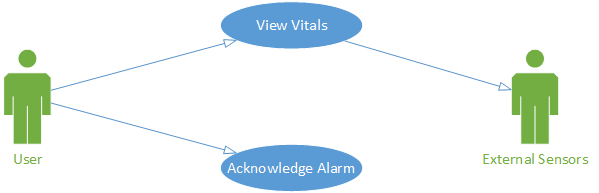
\includegraphics[width=\textwidth]{../design/use_cases_graphical.png}
	\caption{Use case diagram}
	\label{fig:useCases}
\end{figure}

\textbf{Use Case \#1: View Vital Measurements } \\
In the first use case, the user views the basic measurements picked up by the
sensors connected to the device. \\
During normal operation, once the device is turned on by the user, the system
records the value output by each sensor. This raw value is linearized and 
converted into a human-readable form. Finally, this value is displayed onscreen. \\

Three exceptional conditions were identified for this use case: 
\begin{description}
\item [One or more of the expected sensors is not connected:] If this occurs, the measurements taken by the device may be erratic. At the present moment, no action will be taken in such events. Later revisions may address the issue
\item[A measured value is outside 5\% of the specified normal range:] In this case, a warning signal will flash as an indication of the warning condition
\item[A measured value falls outside 10\% of a specified "normal" range:] In this case, an audible alarm will sound to indicate the alarm condition
\end{description}

\textbf{Use Case \#2: Acknowledge Alarm} \\
In the second case, the system is in an alarm state. The user acknowledges
the alarm condition by pressing a button. \\
Upon pressing the button, the system silences the audible alarm. Any visual warnings continue to flash during the silenced period. If a specified amount 
time passes and the sensor reading(s) continue to maintain an alarmed state,
the audible alarm will recommence.\\ 

No exceptional conditions were identified for this use case.\\


\subsection{Software Implementation  Jon}


\subsubsection{Top level design Jon}

%- User use cases  (need to fix)
%  + Take measurements
%  + Acknowledge alarm
%- High level blocks
%  + Functional decomposition
%    o User
%    o Stellaris board
%    o External Sensors
%  + System Architecture (need to flip inheritance arrows and composition arrow)
%    o Discuss shared data
%    o Discuss TCB->Schedular composition
%    o Discuss TCB->task inheritance
%    o Interaction with hardware
%- Implementation in C
%  + Scheduler
%    o Has queue of TCBs
%    o Runs each with minor cycle delay
%      - Timebase
%        o Specifies major/minor cycle
%  + Tasks
%    o Global data is declared in a header file, globals.h and shared with everyone
%    o Get their own file and header file
%    o Own data is hidden from rest of program, single pointer exposed
%    o Every task gets an initialization to initialize data

The design process began by identifying the use cases and actors involved with the system.  In the specified system, the user interacts with the system in one of two ways:
\begin{enumerate}
  \item The user can view their vitals
  \item The user will acknowledge an alarm condition to silence the alarm
\end{enumerate}
In order for a user to view their vitals, the system will have to interact with some external sensors.  Specifically, the system will interact with blood pressure, temperature, and pulse rate sensors.  A graphical depiction of this is shown in Figure~\ref{fig:use}.

\begin{figure}
    \centering
    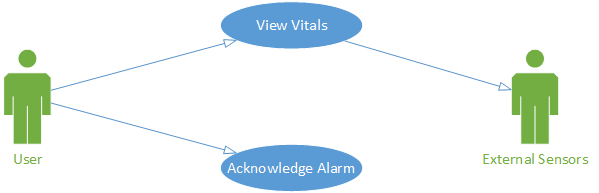
\includegraphics[width=\textwidth]{../design/use_cases_graphical}
    \caption{Use-Case Diagram}
    \label{fig:use}
\end{figure}

After understanding how the user would interact with the device, the system was
functionally decomposed into high-level blocks as shown in
Figure~\ref{fig:func}.  The main system control is located in the CPU, which
controls all data flow into and out of the peripheral devices.  The OLED
displays the user's current vitals including blood pressure (systolic and
diastolic), temperature, and pulse rate.  In the future external sensors will
be added, but for now the values are simulated using the CPU.  The CPU also
controls three LEDs colored green, yellow, and red.  These LEDs are used to
inform the user on the current state of their vitals as well as the state of
the device.  Under normal circumstances, the green LED will be lit.  If the
users' vitals fall outside of a specified range, the red LED will flash at a
specified rate, dependant on which vital is out of range.  If the battery is
low, the yellow LED will be illuminated.

\begin{figure}[h]
    \centering
    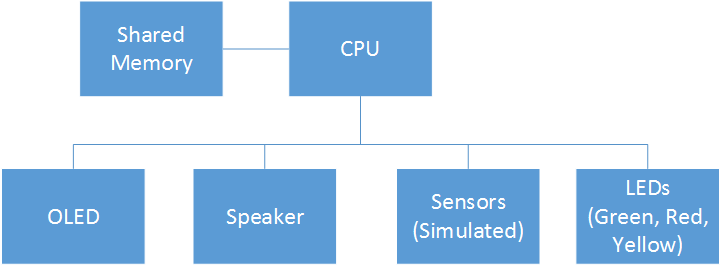
\includegraphics[width=\textwidth]{../design/Functional_decomposition}
    \caption{Functional Decomposition}
    \label{fig:func}
\end{figure}

Next, the system architecture was developed (Figure~\ref{fig:arch}).  At a high
level the system works on two main concepts, the scheduler and tasks.  Tasks
embody some sort of work being done, and the scheduler is in charge of
determining the speed and order in which the tasks execute.  The system has
several tasks, each with their own specific job.  For modularity reasons, each
task should have the same public interface and the scheduler should be able to
run each task regardless of that specific tasks job or implementation.  Thus
the task concept is abstracted into a Task Control Block (TCB), and the
scheduler maintains a queue of TCBs to run.  The TCB abstraction is shown in
Figure~\ref{fig:arch} using inheritance, and the fact that the scheduler has a
queue of TCBs is shown with composition.  The core functionality of the system
was divided into the following five main tasks:
\begin{itemize}
  \item \textbf{Measure Task} - In charge of interacting with the blood pressure, temperature, and pulse sensors (simulated)
  \item \textbf{Compute Task} - Converts sensor data into human readable format
  \item \textbf{Display Task} - Displays the measurements on the Stellaris OLED
  \item \textbf{Warning/Alarm Task} - Interacts with the red, yellow, and green LEDs, as well as the speaker to annunciate warning and alarm information
  \item \textbf{Status Task} - Receives battery information from the device
\end{itemize}
Each of these tasks interact using the shared data shown in Figure~\ref{fig:arch}. 

\begin{figure}
    \centering
    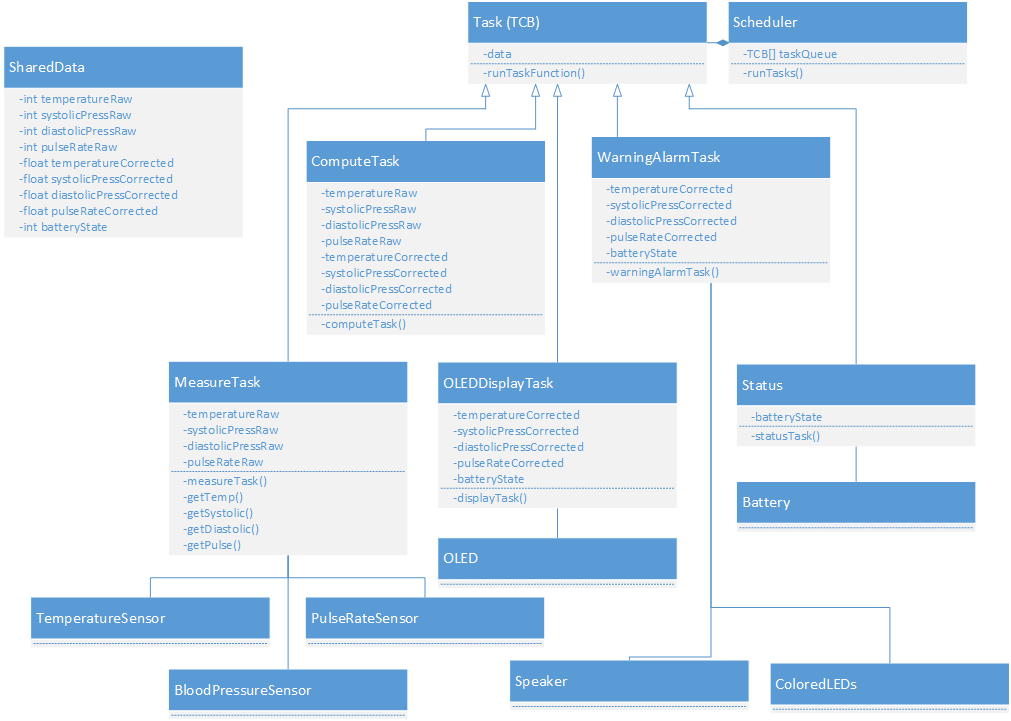
\includegraphics[width=\textwidth]{../design/System_Architecture}
    \caption{System Architecture Diagram}
    \label{fig:arch}
\end{figure}

After developing the system architecture, the design needed to be translated into the C programming language.  The design manifested in a multifile program consisting of the following source files:
\begin{itemize}
  \item \textbf{globals.c/globals.h} - Used to define the Shared Data used among the tasks
  \item \textbf{schedule.c/schedule.h} - Defines the scheduler interface and it's implementation
  \item \textbf{timebase.h}
\end{itemize}

\subsubsection{low level design  Jarret}

implementation details here. Tasks, scheduler, etc. Control diagram goes here, activity diagram, etc.

\section{Presentation, Discussion, and Analysis of the Results}

Based upon the execution of your design, present your results. Explain them and what was expected, and draw any conclusions (for example, did this prove your design worked).

In addition to a detailed discussion and analysis of your project and your results, you must include all the answers to all questions raised in the lab.
\subsection{results}
The project was completed and demonstrated on January 29, 2014. \\

Demonstration of the system to the interested parties showed that the system met the requrements initially presented at the onset of the lab project.
Testing of the system prior to demonstration also verified that the system met the specifications listed in Section~\ref{sec:designSpec}. \\
Additionally, during the demonstration, to show that several warning features worked as expected, source code was temporarily modified to speed up the progression of the system through various warning states. These changes were simple to execute and caused the desired effect on the system without causing unwanted abberrant behavior. Reverting the source code was similarly intuitive.
During the actual coding and implementation of the design, remarks were made several times about the ease of execution during that phase of the project. After the initial high level Design phase, very few changes were made, or required, to the functional design or system architecture.\\

Using an oscilloscope, the runtimes of each task were empirically determined. The results are given in Table~\ref{tab:taskRuntimes}.

\begin{figure}[h]
	\centering
	\begin{tabular}{|l|r|} 
		\hline
		Task & Runtime ($\mu$s) \\ \hline
		Measure & 23.4 \\ \hline
		Compute & 55.4 \\ \hline
		Display & 22900.0 \\ \hline
		Warning & 27.4	\\ \hline
		Status & 5.6	\\ \hline
	\end{tabular}
	\caption{Empirically determined task runtimes\label{tab:taskRuntimes}}
\end{figure}


\textbf{Answers to the last three questions in the list of items to include in the project report:} \\
\emph{You don't find the stealth submarine. That's why they are so expensive; at that cost, you take great pains to never lose one.\\
A helium balloon always rises. It just rises upside-down. \\
If you really managed to lose the stealth submersible, you first have to tell the government, which will deny it has any stealth submersibles, then you have to comb the seven seas until your comb hits the sub.}
 
\subsection{discussion of results  Jon}

\subsection{Analysis of any Errors}
The project was completed without any residual errors or unsolved problems. See the following section for analysis of issues encountered while working on the project itself.

\subsection{Analysis of problems and issues encountered and what efforts were made to identify the root cause of any problems  Jarrett}

%State any problems you encountered while working on the project. If your project did not work or worked only partially, provide an analysis of why and what efforts were made to identify the root cause of any problems. \\

%Some points to bring up: did not enable the GPIO bank (caused OLED display to not work), could not get switch to work (solved by understanding that switch required pull up). P or J can talk about design solutions that did not work. On the whole, we had problems with going too deep, too quickly.

The medical instrument design in this project was completed and tested succesfuly to meet all the requirements, the designers did face a number of errors and difficulties in the process. Most of the challanges faced in this design were in implementing the inputs and outputs from the ARM micro processor. In this implementation, the students orginally had consulted the driver library documentation and found how to enable a general purpose input output (GPIO) pand, GPIO pin, and how to read from a GPIO pin. However, when the code to enable a GPIO pin was executed, the execution of tasks within the scheduler froze completely until a reset. This problem was caused by the students failure to enable the peripheral bank that the GPIO pins existed on. After learning how to do this, code was added to enable the peripheral and the task execution no longer froze on enabling a pin.

Another problem encountered by the design team was that initially after setting up a GPIO pin as an input to take a button press from the Stellaris test board, pressing the button did not have the intended effect. The push button did not change the state of the input. The students were originally perplexed and tried a number of solutions to this problem. Testing indicated that the code for the GPIO input was correct as a 3.3 V signal directly to the pin could trigger the intended event on the input. Eventualy it was found that to use the push button switch the GPIO pin's pad must be configured to accept a pull up resistor type of input.

All problems were solved before demonstrating the product to the interested parties. As such, the final design did not have any errors.

\section{Test Plan}

To ensure that this project meets the specifications listed in 
section~\ref{sec:designSpec}, the following parts of the system must be 
tested: 

\begin{itemize}
	\item Vitals are measured and updated every five seconds
	\item System properly displays corrected measurements and units properly
	\item System enters, indicates, and exits the proper warning state for blood pressure, temperature, pulse, and battery
	\item System enters and exits the alarm state correctly
	\item Alarm is silenced upon button push
	\item Alarm recommences sound after silencing if system remains in alarm state longer than slilence period
\end{itemize}

Additional tests to determine the runtime of each specific task are also required.

\subsection{Test Specification Jon}

Annotated description of what is to be tested and the test limits.  This specification quantifies inputs, outputs, and constraints on the system.  That is, it provides specific values for each. 

Note, this does not specify test implementation...this is what to do, not how to do it.

\subsection{Test Cases  Jarrett}

The students begin testing by examining if the alarm sounds at the proper time. This is initialy tested by disabling the functions that simulate measurements being made on each of the data measurements, and setting their initial values to be either within the alarm range or outside of the alarm range. The warning states were also initialy tested this way. The initial values for raw data below were used to test the normal state of the machine because each falls within the acceptable range of measurements for corrected data also given below that does not require a warning.
\begin{figure}[h]
	\centering
	\begin{tabular}{|l|c|r|} 
		\hline
		Data & Initial Raw Value & Acceptable Range \\ \hline
		Temperature & 42 & 36.1 C to 37.8 C  \\ \hline
		Pulse & 25 & 60 to 100 beats per minute \\ \hline
		Systolic Pressure  & 10 & less than 120 mm Hg \\ \hline
		Diastolic Pressure & 10 & less than 80 mg Hg	\\ \hline
	\end{tabular}
	\caption{Initial values and System ok parameters\label{tab:testing initil values}}
\end{figure}
	
Using these initial values, the code was programmed onto the Stellaris board. Correct operation was verified by the alarm not sounding, and the red led being off, indicating that no warning state was in effect. In addition the green led was on indicating a normal state. Next the students varried one parameter at a time to be outside of the acceptable range by more than 10\%. Starting with the temperature being set to an initial raw value of 50, the alarm was verified by hearing the aural annunciation coming from the system. In addition, the temperature warning stat was also in effect. This means that the green led was off and the red led was blinking. To verify correct operation we needed to make sure the led was blinking with a period of 1 second. The correct flashing pattern was verified by counting the number of times the led flashed in 6 seconds. In this case, for temperature, the led flashed 6 times in 6 seconds indicating a 1 second period, and correct operation. After this test, the temperature value was returned to 42 and the Pulse was instead set to 45. The same methods were used to verify that the alarm and warning states for pulse rate were working correctly, but this time the warning led turned on 3 times in 6 seconds indicating a 2 second period which is the intended period of flashing. The pulse rate was then returned to 25 and each pressure reading was checked for correct operation individualy by being set to an initial raw value of 100. Once again, the green led started off because the system was not in a nirmal state. The alarm was sounding due to the extremely high blood pressure measurements, and the red warning led flashed 12 times in 6 seconds indicating the correct period of .5 seconds for a blood pressure warning. In addition to testing the validity of each warning state and alarm state, the acknowledgement of the alarm was also tested during each of these tests. This was tested by hitting the acknowledge button once during each measurements test. During each test, hitting the acknowledge button turned the alarm sound off for a short time, as intended. 

Next the measuremet simulation functions were tested. This was done by re-enabing each one that had been disabled from the previous test one at a time. The initial raw values were again set to the values in Figure 5. When each measurement was reenabled, the students could watch the temperature change at each major cycle using the oled display. Since the oled display indicated that the corrected temperature went up .75 degrees on a major cycle then down 1.5 degrees on the next, the temperature measurement was working as intedned. This situation also gave the students an opprotunity to verify that the warning and alarm states initiated as the temperature fell out of the acceptable range. The Led began flashing with a 1 second period after a few major cycles, then the alarm began sounding, indicating correct operation. Since temperature was working correctly, the temperature measurment function was once again disabled and the pulse rate measurement function was re-enabled. The oled display indicated that the pulse rate was increasing by 3 on a major cycle then falling by 6 on the following major cycle. This was consistent with the intended design. The alarm and warning being initiated as the pulse rate fell. The pulse rate measurement was then disabled and each blood pressure measurement was re-enabled individualy for testing. The Systolic pressure began by rising 4 mm Hg on a major cycle then falling 2 mm Hg on the next, and the Diastolic pressure by rising 3 on a Major cycle and falling 1.5 on the next, this was consistent with our design. The warning and alarm states were activated as each passed its threshold and the red led was blinking with a period of .5 seconds. The warning led was also tested in the case that all warning states were active. To do this all initial values were set to 100. In this case, as designed by the students, the red warning led indicated the fastsest blinking warning with a .5 second period. 

The final bit of testing preformed on the system was timing each task within the system. This was done by adding a general purpose output pin in our scheduler code. This output was set high right before the execution of a task, and set low immediately after the execution of the task. An oscciloscope was then attached to this output pin and set to trigger on a positive edge. The cursors were then used to measure the amount of time the signal was high in each cycle.

\section{Summary and Conclusion}

\subsection{Final Summary}
The students began creating their medical instrument through a rigorous design process at different levels of detail. The students then continued work by implementing their design in C code for the ARM Cortex A3 microprocessor. Next the code was tested and debugged using the IAR workbench debugging tool, as well as visual queues programmed into the design. Finally, after verifying that the system worked as specified, it was presented to the instructor.

\subsection{Project Conclusions}
This project contained 3 major phases, the design, implementation, and testing steps. The students were immediately introduced to using the unified modeling language(UML) to design embedded systems. This is the first time many students will have used UML for system design which caused some confusion and difficulty. In the end through the use of the UML guidelines for design, the students were able to implement their system in code for the Texas Instruments Stellaris EKI-LM3S8962 much more quickly and with far fewer errors than if they had spent less time in the design phase of this project. 

Effective design tools allowed the students to quickly implement their embedded system in C code for an ARM Cortex A3 processor, and move onto the testing phase of the project quickly. Unfortunately, while testing the students encountered a number of problems in using the pwm and general purpose input and output signals. After consulting the documentation for the Stellaris kit and solving their input/output problems, they began testing thri design using visual and audio queues, the IAR embedded workbench debugger, and a few specifically programmed debug features. After the results of the testing verefied the design to be working correctly, the students proceeded to present their medical instrument to their instructor.



\pagebreak
\appendix

\section{Breakdown of Lab Person-hours (Estimated)}

\begin{tabular}{|l|*{4}{r|}}
	\hline
	Person & Design Hrs & Code Hrs & Test/Debug Hrs & Documentation Hrs \\ \hline
	Patrick & 15 & 7 & 2 & 9  \\ \hline
	Jarret & x & x & x & x  \\ \hline
	Jonathan & x & x & x & x  \\ \hline
\end{tabular}

~\\

By initializing/signing above, I attest that I did in fact work the estimated number of hours stated. I also attest, under penalty of shame, that the work produced during the lab and contained herein is actually my own (as far as I know to be true). If special considerations or dispensations are due others or myself, I have indicated them below.

\pagebreak

\section{Source Code}

Source code for this project is provided below.

\subsection{The first part}
% \lstinputlisting{source.c}

\subsection{The second part}
% \lstinputlisting{source.c}

\end{document}
